\chapter{Training}
\label{ch:training}

In diesem Kapitel wird der detaillierte Trainingsablauf mit all seinen Hyperparametern beschrieben.
Das Training stellt eine Form von Transfer Learning zur Multi-Label-Klassifikation dar.
Es werden ausschließlich vortrainierte Modell verwendet und angepasst.
Alle Rechenergebnisse basieren auf einem einheitlichen Trainingsprotokoll, welches es ermöglicht, die Ergebnisse zu vergleichen und zu reproduzieren.
%Die Implementationen basiert auf den Open-Source Bibliotheken PyTorch, Torchvision (für Bild- und Videoverarbeitung) und Ignite (als Framework für Training).

Dazu werden alle möglichen Hyperparameter aufgelistet, kategorisiert und eine Entscheidungsfindung für die Wahl erläutert.
Anschließend werden alle vorgelagerten Prozesse, der eigentliche Trainingsablauf, sowie nachgelagerte Prozesse veranschaulicht.

\begin{tcolorbox}[title=Todo]
    \begin{itemize}
        \item Wireframe: Relabel (Beispiel von Fehlerhaftem Sample)
    \end{itemize}
\end{tcolorbox}

Das Training von Deep-Learning-Modellen ist durch die Wahl etlicher Hyperparameter geprägt.
Einige können mithilfe gängiger Best Practices, andere durch manuelle Verfahren oder durch iteratives Ausprobieren bestimmt werden.
Der hier vorgestellte Trainingsablauf lässt sich in vier Parametergruppen gliedern:

\begin{description}
    \item[Sampling-Parameter] Die in \autoref{subsec:hyperparameter} vorgestellten Parameter $\gamma_s$ (Auflösung), $\gamma_\tau$ (Samplingrate) und $\gamma_t$ (Anzahl der Frames) sind Teil der Evaluation und werden in verschiedenen Experimenten ausprobiert.
    Der Richtwert $\gls{tld:Theta}_\text{train}$, der die Maximalzahl von Samples pro Klasse beschränkt, wird zunächst auf 100 gesetzt, in späterem Experimenten zur weiteren Optimierung jedoch erhöht.
    \item[Hardware-abhängige Parameter]
    Zu dieser Gruppe gehört \zB die Batch-Größe, die durch die Speicherkapazität der Grafikkarte beschränkt wird.
    In \autoref{subsec:hardwareeinschrankungen} wird der Umgang mit begrenzten Speicher beschrieben und wie die Parameter gewählt werden.
    \item[Modell-abhängige Parameter] Zu dieser Gruppe zählt vorrangig die zu wählende Lernrate, die bestimmt in welchem Maß die Modellparameter angepasst werden.
    Auch hierzu wird in \autoref{subsec:vorkehrungen} ein Verfahren zur Findung erläutert.
    \item[Sonstige Parameter] Alle übrigen Parameter werden auf der Grundlage vorherrschenden Best Practices oder den Implementationsdetails des jeweils vortrainierten Modells bestimmt.
\end{description}

\section{Vorbereitung}
\label{sec:vorbereitung}

Bevor das eigentliche Training startet, müssen Parameter wie Batch-Größe und Lernrate durch iterative Prozesse in jedem Experiment bestimmt werden.
Ebenfalls ist eine manuelle Einsicht in die Daten durch das Plotten zufälliger Samples (wie in \autoref{fig:sample_example}) hilfreich, um sicherzustellen, dass alle Pre-Processing-Schritte funktionieren.

\subsection{Hardwareeinschränkungen und Bestimmung der Batch Größe}
\label{subsec:hardwareeinschrankungen}

Die Experimente werden mithilfe einer einzelnen \gls{gpu} (Modell Tesla P100-PCIE-16GB \bzw Tesla V100-SXM2-16GB) durchgeführt.
Da die Feature-Maps proportional zu den Sampling-Parametern $\gamma_s$ und $\gamma_t$ wachsen, kann schon bei einer kleinen Batch-Größe das Speicherlimit der Grafikkarte erreicht werden.

Als Antwort auf diese Einschränkung werden zum einen die Modelle konsequent mit einer Genauigkeit von 16 Bit (Half Precision) statt der gängigen 32 Bit trainiert.
Zum anderen wird die Batch-Größe, als zentraler Parameter, der Einfluss auf Trainingsdauer und Performance hat, justiert.
Größere Batches liefern stabilere Gradienten und meist bessere Ergebnisse, verlangsamen jedoch das Training da mehr Epochen bis zur Konvergenz nötig sind (\cite{Gugger20}).
Als Richtwert wird eine Batch-Größe von 64 festgelegt.
Dieser Wert orientiert sich am Transfer Learning in~\cite{Feichtenhofer18} und stellt zugleich sicher, dass in jedem Update-Schritt potenziell alle 32 Klassen, sowie Background-Samples repräsentiert sein können.

Da eine Batch-Größe von 64 bei den allermeisten Experimenten nicht in den \gls{gpu}-Speicher passt, wird zunächst die maximal mögliche Batch-Größe mittels Binärer Suche bestimmt.
Ist die maximale Batch-Größe größer oder gleich dem Richtwert, wird der Richterwert als Batch-Größe übernommen.
Ist sie kleiner als der Richtwert, wird als weiteres Hilfsmittel eine Gradient Accumulation genutzt.
Diese stellt sicher, dass die Gradienten der kleinere Batches solange für den Backpropagation-Schritt aufsummiert werden bis der Richtwert von 64 Samples wieder erreicht ist.
Die eigentliche Batch-Größe wird dazu auf den größten gemeinsamen Teiler aus maximaler Batch-Größe und Richtwert abgerundet.
Sollte die maximale Batch-Größer die untere Grenze von 8 unterschreiten, muss in letzter Instanz auf das Training vorderer Layer verzichtet werden, um so zusätzlich Speicher zu sparen.
Die Auswahl über die Anzahl der Layer, die in diesem Fall eingefroren werden, passiert ebenfalls iterativ und wird entsprechend in den Experimenten angegeben.


\subsection{Bestimmung der Lernrate}
\label{subsec:vorkehrungen}

Für die Wahl der passenden Lernrate wird ein iterativer Test für verschiedenen Lernraten durchgeführt.
Der Test probiert verschiedene Lernraten aus und plottet diese gegen den resultierenden Fehler (in diesem Fall Binary Cross Entropy), wie \autoref{fig:lr-finder} zeigt.
Dabei wird diejenige Rate als Lernrate empfohlen, deren Abstieg maximal ist~\cite{Smith15}.

\begin{figure}
    \centering
    \bigimage{img/lr_finder}{0.65\textwidth}
    \caption{Lernraten-Finder mit markierter Empfehlung aus~\cite{Gugger20}}
    \label{fig:lr-finder}
\end{figure}

Da im Folgenden ausschließlich Transfer Learning angewandt wird, wird die Lernrate nicht als skalarer Wert, sondern ein Intervall definiert.
Mit sogenannte diskriminativen Lernraten (discriminative fine-tuning~\cite{Howard18}) erhalten vordere Layer eines Netzes kleinere Lernraten als hintere Layer.
Dem liegt die Idee zugrunde, dass die vortrainierten Low-Level-Features der vorderen Layer eine allgemeinere Gültigkeit haben und weniger an die neue Domäne angepasst werden müssen, als die High-Level-Features hinterer Layer.
Die diskriminativen Lernraten ergeben sich aus einem Intervall um den empfohlenen Richtwert, wobei das gesamte Intervall eine stetig negative Steigung ausweisen sollte.
Im Beispiel aus \autoref{fig:lr-finder} wäre $[1e^{-03}, 1e^{-01}]$ ein mögliches Interval.

\section{Trainingsablauf}
\label{sec:trainingsablauf}

Allen Experimenten geht die jeweilige Suche nach Batch-Größe und Lernraten voraus.
Anschließend findet das eigentliche Training nach einem wie folgt beschriebenen, fest definierten Ablauf statt.

\subsection{Trainingsschleife}
\label{subsec:trainingsschleife}

Alle Experimente folgen dem gleichen Schema in Form eines Trainings-Loops:
\autoref{fig:train-loop} zeigt den Algorithmus des Trainings-Loops, in der pro Epoche eine Schleife durchlaufen wird:

Zunächst werden Batches aus dem Trainingsset gesamplet, bevor der Vorwärts- und Rückwärts-Pass des \gls{har}-Modells durchlaufen wird.
Aus den Scores (Predictions) des Vorwärtspasses, werden mithilfe der Ground-Truth-Labels $y$ die Fehlerwerte (Losses) berechnet.
Scores und Losses werden intern zwischengespeichert und in einer separaten \code{Evaluator}-Komponente zwischengespeichert, die pro Epoche Metriken zur Bewertung des Modells erfasst und loggt.

Sobald alle Trainingsdaten einmal verarbeitet wurden, werden analog die Validierungsdaten gesamplet, die allerdings nur den Vorwärtspass des \gls{har}-Modells durchlaufen.
Diese resultierenden Scores und Losses werden analog im \code{Evaluator} zwischengespeichert.

Am Ende einer Epoche wird anhand der Metriken geprüft, ob das Modell overfittet.
Ist letzteres der Fall, kann der Trainings-Loop vorzeitig abgebrochen werden (Early-Stopping).

\begin{figure}[htbp!]
    \centering
    \bigimage{fig/training}{0.95\textwidth}
    \caption{Sequenzdiagramm: Trainings-Loop}
    \label{fig:train-loop}
\end{figure}

Nach dem Durchlauf werden alle Metriken, Hyperparameter, sowie die besten Modellgewichte (Checkpoints) und der Quellcode an einen persistenten Cloud-Speicher übermittelt, sodass keine Informationen verloren gehen.
Auch die Scores und Losses werden mit weiteren Daten zur Identifizierung der jeweiligen Samples in Form einer \gls{csv}-Datei übermittelt.
Die Speicherung von Scores und Losses dient letztlich der Fehleranalyse in \autoref{sec:nachgang}.

Zudem geht dem beschriebenen Ablauf der Schritt des Scheduling in jeder Trainingsiteration vorher.
Scheduling meint in diesem Zusammenhang das zeitabhängige Anpassen von Hyperparametern während des Trainings: in diesem Fall der Lernraten.

In allen Experimenten wird hierzu ein One-Cycle-Schedule~\cite{Smith15} erstellt, der die Lernraten in jedem Iterationsschritt anpasst.
Im ersten Drittel werden die Lernrate von einer 10x kleineren initial Lernrate aus angenähert, während sie sich in den letzten zwei Dritteln wieder auf null abkühlen.
\autoref{fig:one-cylce} zeigt einen exemplarischen Verlauf für die Basis-Lernrate von 0.01.
Diese Praxis verspricht eine schnellere Konvergenz, indem der Optimizer im ersten Drittel mehr Freiheitsgrade bekommt, um nach einem guten Startpunkt zu suchen und lokalen Minima zu entkommen.
In den hinteren Dritteln kann diese Startlösung langsamer optimiert werden als vorher, sodass zu große Sprünge vermieden werden.

\begin{figure}
    \centering
    \begin{subfigure}{.5\textwidth}
        \centering
        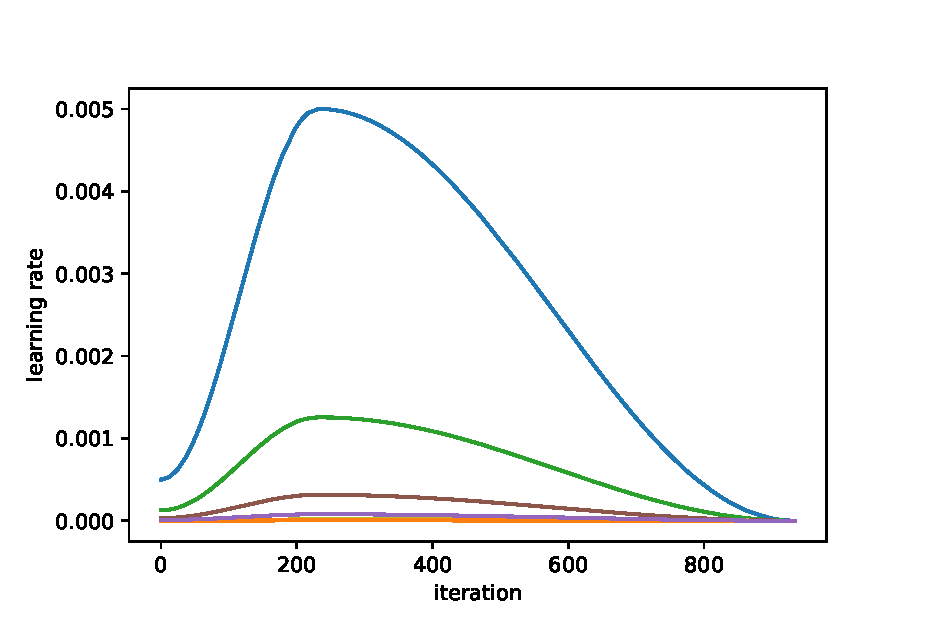
\includegraphics[width=.9\linewidth]{img/06_one_cycle_lin.eps}
        \caption{lineare Skala}
    \end{subfigure}%
    \begin{subfigure}{.5\textwidth}
        \centering
        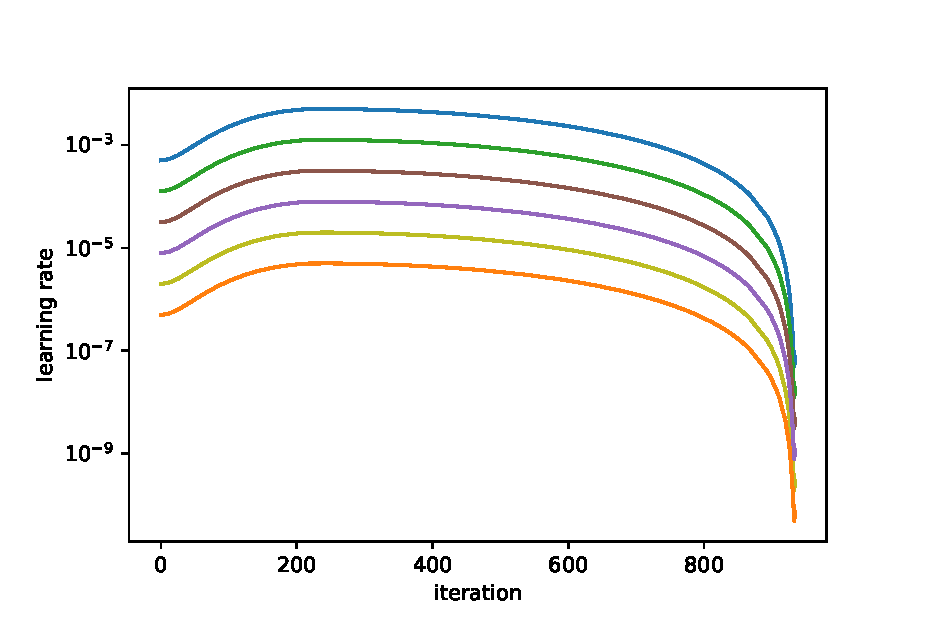
\includegraphics[width=.9\linewidth]{img/06_one_cycle_log.eps}
        \caption{logarithmische Skala}
    \end{subfigure}
    \caption{One Cycle Schedule für diskriminativen Lernraten}
    \label{fig:one-cylce}
\end{figure}

Der Backward-Pass basiert auf einem Adam-Optimierer~\cite{Kingma14} mit der Standardkonfiguration nach~\cite{Gugger20}.
Die Anzahl der Epochen wird in der ersten auf 10 beschränkt, was zum Initialisieren und einen einfachen Benchmark ausreicht.
In späteren Experimenten werden meist weniger Epochen verwendet, da das Modell bereits auf ähnliche Daten angepasst ist.

\subsection{Reaktive Änderungen}
\label{subsec:reaktive-aenderungen}

Wie schnell das Modell innerhalb des Trainings-Loops lernen kann ist letztlich auch von der Architektur selbst abhängig.
Die Zykluslänge im One-Cycle-Scheduling ist definiert durch die Anzahl der Epochen.
Sollte ein Modell im Zuge des Trainings massiv overfitten, ist es oft hilfreich den Durchlauf neu zu starten und dabei die Zahl der Epochen auf diejenige Epoch zu beschränken, in der zuvor das Overfitting begann~\cite{Gugger20}.

Eine weitere Reaktion ist der Einsatz von L2-Regularisierung, die die Summe der Modellparameter in die Fehlerfunktion einfließen lässt.
Das Maß des Einflusses wird durch eine Weight-Decay-Rate bestimmt, die, sofern nicht anders hervorgehoben, immer aus den Hyperparametern des vortrainierten Modells übernommen wird.

\subsection{Metriken}
\label{subsec:metriken}

Die in jeder Epoche erhobenen Metriken geben Aufschluss darüber, wie gut das aktuelle Modell auf dem jeweiligen Datenset performt und wie sich die Performance zeitlich entwickelt.
Während des Trainings werden folgende globalen Metriken erfasst:

\begin{itemize}
    \item Balanced Accuracy: $BA = \frac{1}{2} ( \frac{TP}{TP + FN} + \frac{TN}{FP + TN} )$
    \item Precision: $PR = \frac{TP}{TP+FP}$
    \item Recall: $RE = \frac{TP}{TP+FN}$
    \item F1-Score: $F1 = \frac{2 \cdot TP}{2 \cdot TP + FP + FN}$
    \item Area Under the Receiver Operating Characteristic Curve (AUROC)
\end{itemize}

Die oberen vier Metriken, werden jeweils pro Klasse erhoben, um später Aussagen über die individuelle Lernbarkeit einer einzelnen Klasse treffen zu können.
Darüber hinaus wird der Durchschnitt über alle Klassen Klasse (macro) oder das direkte Verhältnis auf Basis der klassenübergreifend aufsummieren Faktoren (TP, FP, etc.) erfasst (micro).
Sofern nicht anders hervorgehoben, sind die im weiteren Verlauf vorgestellten, skalaren Metrikwerte immer Macro-Werte.

\section{Verifikation}
\label{sec:nachgang}

Im Phase 3 der Experimente werden basierend auf den vorhergegangenen Experimenten potenzielle Daten-Fehler verifiziert.
Da aus Zeitgründen nicht alle Samples kontrolliert werden können, wird sich auf diejenigen Samples beschränkt, die mit erhöhter Wahrscheinlichkeit fehlerhaft gelabelt sind.
Hierfür wird auf die während des Trainings persistierten Scores und Losses zurückgegriffen, die in einem Fehlerbericht persistiert sind.
Mithilfe des Fehlerberichts genügt es, nur die Samples mit den höchsten Loss-Werten manuell zu kontrollieren.

Schon während des Samplings (\autoref{subsec:segmentierung-und-sampling-strategie}) wird jedes Sample mit einer eindeutigen ID verknüpft, die sich aus dem zugehörigen Match und der Startmarkierung (in Videozeit) zusammensetzt.
Mithilfe der ID können die Annotationen auch nachträglich aus der JSON-Datenbank geladen und die Scores mit den Ground-Truth-Labels des Samples verglichen werden.
Dabei werden die Samples der besten Epoche für alle Datensets absteigend nach ihrem Loss sortiert und mithilfe eines Relabel-Tools verifiziert und im Fehlerfall \ggf korrigiert.
Wird ein Fehler entdeckt kann dieser auf dreierlei Weisen behoben werden:

\begin{description}
    \item[Zusätzliche Aktion] Eine Aktion, die in den Annotationen vorher nicht erfasst war, ereignet sich im Videobild.
    Die Aktion kann als Tupel, bestehend aus Label und Zeitfenster, der Datenbank hinzugefügt werden.
    Dieser Fall tritt \zB auf, wenn eine Wiederholung gezeigt wird.
    \item[Verschobene Aktion] Eine Aktion, tritt im Videobild früher oder später auf, als es in den Ground-Truth-Daten dokumentiert ist.
    In der Datenbank findet sich genau die gesuchte Aktion, deren Zeitfenster jedoch nicht übereinstimmt.
    In diesem Fall kann die \code{segment}-Eigenschaft der Annotation in der Datenbank geändert werden.
    \item[Verdeckte Aktion] Eine Aktion, die stattgefunden hat, ist im Kamerabild nicht zu sehen und muss aus der Datenbank gelöscht werden.
\end{description}

Das Relabel-Tool speichert die Änderungen nicht direkt in der JSON-Datenbank, sondern in einer zusätzlichen Datenstruktur, die ausschließlich die Datenbank-Transaktionen enthält, die für ein Update notwendig sind.
Zur Laufzeit wird die JSON-Datenbank in den Arbeitsspeicher geladen und kann dort optional mithilfe der Transaktionsdatei angepasst werden.
Um die Transaktionen endgültig zu speichern, kann die angepasste Datenbank mit einer neuen Versionsnummer wieder auf dem Dateisystem persistiert werden.

Die Verifikation folgt einem definiertem Protokoll:
Sind alle Experimente einer Phase abgeschlossen, wird zunächst eine neue Transaktionsdatei erstellt.
Für jedes der Experimente wird das Relabel-Tool mit den persistierten Score- und Loss-Werte des Fehlerreports initialisiert.
Das Relabel-Tool erhält ebenfalls Zugriff auf die bestehende JSON-Datenbank.
Die Samples werden absteigend nach Loss-Wert sortiert und dem Nutzer interaktiv präsentiert.
Der Nutzer kann die einzelnen Annotationen des Samples ändern oder löschen oder eine neue Annotation hinzufügen.
Jede dieser drei Operationen lässt sich in Form einer Transaktion in einer \gls{csv}-Datei speichern.
Nach der Verifikation eines Experiments werden die Transaktionen separat gespeichert, dann auf die Datenbank angewendet und dann die Datenbank in einer neuen Version gespeichert.
Die geänderten Annotationen werden zudem als verifiziert in der Datenbank markiert, sodass der Nutzer die gleichen Fehler nicht mehrmals im Relabel-Tool vorgeschlagen bekommt.

Eine weitere Funktion des Fehlerreports besteht darin nach Auffälligkeiten in den Daten zu suchen:
Es kann der durchschnittliche Fehler pro Video ermittelt werden und Ausreißer können mit einem z-Test identifiziert werden.
Diese Ausreißer sind \zB Videos mit vielen Kodierungsfehlern oder einer nicht konstanten Abspielgeschwindigkeit, die im Rahmen dieser Arbeit nicht zum Einsatz kommen sollten, da sie die Qualität des Datensets im Allgemeinen beeinträchtigen.
Falls die Qualität dieser Videos inakzeptabel ist, werden sie manuell aus der Datenbank entfernt.
